% Nama Kelompok: Kelompok 1
% Kelas: D4 TI 1A
% Anggota: 1. Dezha Aidil Martha 1174025
% 		   2. Habib Abdul Rasyid 1174002
% 		   3. Muhammad Tomy Nur Maulidy 1174031
% 		   4. Nico Ekklesia Sembiring 1174095
% 		   5. Felix Setiawan Lase 1174026
% 		   6. Damara Benedikta Siolemba 1174012


%ASCII
	\section{ASCII}
		\subsection{Definisi ASCII}
		berdasarkan artikel yang ditulis oleh hieronymus \cite{hieronymus1993ascii}
	ASCII atau American Standard Code for Information Interchange merupakan sebuah pengkodean berstandar Internasional yang berupa kode huruf dan simbol, seperti Hex dan Unicode dan juga merupakan simbol tambahan dari database. ASCII bersifat universal contohnya 124 untuk karakter "|". ASCII selalu digunakan oleh komputer dan alat komunikasi yang lain untuk menunjukkan teks.
    Dalam kode ASCII mempunyai komponen komponen bilangan biner yang berjumlah 7 bit. Kode ASCII berfungsi untuk mewakili karakter angka ataupun huruf di dalam komputer. Sebuah pengkodean ASCII dari Afabet Fonetik Internasional atau IPA dirancang untuk semua bahasa. Skema ASCII yang akan dibuat serupa dengan simbol IPA dasar sehingga akan banyak simbol yang memiliki makna jelas dan banyak simbol yang sama dengan skema yang lain. Prinsip dasarnya merupakan spectrally dan tempor berbeda yang memiliki sifat fonemik.
    Dalam beberapa bahasa harus memiliki simbol dasar yang terpisah. Dalam kebanyakan kasus, simbol dasar terdiri dari aconcatenation dari simbol IPA. Dengan demikian mudah untuk mengenali simbol dasar fonemik dan membandingkan suara fonetik lebar yang sama di seluruh bahasa. Bahasa nada telah diacritics dan diterapkan pada simbol fonem vokal untuk mengidentifikasi fonem dengan benar dalam bahasa-bahasa ini. Allophonic variasi karena koartikulasi dan stress kontek stual dapat diberi label.
	Simbol dasar Ada kemungkinan bahwa beberapa suara ucapan yang merupakan fonemiK.Satu dar iyang lain hilang dari versi sekarang. Diharapkan setiap kelalaian akan terjadi dikoreksi dalam versi Worldbet berikutnya, dan menggunakan metode standar untuk membangun simbol yang baru. Alfabet Fonetik Internasional dikembangkan di Indonesia pada tahun 1888 dan ada beberapa kali revisi kedalam bentuknya yang sekarang. Ini mewakili 105 tahun pengalaman dengan meletakkan simbol untuk setiap suara dalam semua bahasa yang dikenal di dunia. 
	Representasi dan perbedaan antara variasi alofonik dan suara base form sejati telah terjadi
	bekerja untuk lebih banyak bahasa sejak IPA diformulasikan. 
	tempat untuk memulai untuk multi bahasa pidato database pelabelan eortort.
	Ada beberapa suara yang biasanya tidak termasuk dalam IPA yang telah ditemukan
	berguna untuk memberi label pada corpora ucapan besar seperti TIMIT, SCRIBE, BDSON, dan PHONDAT. Ini
	Upaya modern mengenai bentuk standar ASCII IPA menghasilkan TIMITBET, MRPA, SAMPA, dan
	SAMPA Diperpanjang untuk beberapa nama dari mereka. Huruf fonetik ini dibatasi untuk bahasa Inggris atau bahasa Inggris kebahasa-bahasa Eropa.
	ASCII memiliki jumlah kode sebanyak 255 dengan nilai ANSI ASCII desimal 0 sampai 127 merupakan kode ASCII manipulasi teks sedangkan kode ASCII dengan nilai ANSI ASCII 128 sampai 255 merupakan kode ASCII untuk memanipulasi gambar grafik.
	
		1. Kode yang tidak terlihat seperti kode 8 back space,10 pergantian baris,32 spasi 
		2. sedangkan kode yang terlihat simbolnya seperti numerik atau angka 0...9 abjad a...z karakter khusus.
		3. dan kode yang tidak ada di keyboard tapi tidak dapat ditampilkan, kode-kode ini biasanya untuk kode-kode grafik dengan nilai ANSI ASCII 128 sampai 225.
  

	Berikut contoh tabel berisi karakterk-karakter ASCII.
\begin{table}[H]
\begin{tabular}{|c|c|c|c|c|}
hline
Karakter & Nilai Unicode (heksadesimal) & Nlai ANSI ASCII(desimal) & Keterangan\\
\hline
NUL & 0000 & 0 & Null(tidak tampak)\\
SOH & 0001 & 1 & Start of Heading(tidak tampak)\\
0 & 0030 & 48 & Angka nol\\
1 & 0031 & 49 & Angka satu\\
2 & 0032 & 50 & Angka dua\\
3 & 0033 & 51 & Angka tiga\\
4 & 0034 & 52 & Angka empat\\
5 & 0035 & 53 & Angka lima\\
6 & 0036 & 54 & Angka enam\\
7 & 0037 & 55 & Angka tujuh\\
8 & 0038 & 56 & Angka delapan\\
9 & 0039 & 57 & Angka sembilan\\
\hline
\end{tabular}
\end{table}

		\subsubsection{Prinsip-Prinsip Umum ASCII}
 	Dalam ASCII dikenal juga Worldbet. Worldbet adalah versi ASCII dari  International Phonetic Alphabet (IPA) dengan tambahan luas simbol fonetik yang saat ini tidak ada di IPA. Worldbet ini dirancang untuk sejumlah besar bahasa termasuk Bahasa India, Asia, Afrika dan Eropa. Pertimbangan suara khusus di masing – masing bahasa ini mengarah pada prinsip bahwa setiap simbol dasar akan mewakili suara ucapan urutan waktu yang berbeda secara spektral. Setiap jenis / r / akan memiliki IPA yang terpisah, bukan r graphemic yang digunakan di beberapa label. Allophones seperti plorives aspirated akan memiliki simbol dasar terpisah dari plosives yang tidak diaspirasikan, mereka adalah fonemik dalam bahasa di pertanyaan, jika tidak mereka akan ditandai dengan menggunakan simbol dasar plus (diakritik). Begitu berbeda secara spektral atau temporer karena secara perseptual berbeda, ketika komponennya didengar dalam isolasi. Vokal digolongkan ke posisi posisi nominal. Hal ini diakui bahwa warna vokal rinci dapat bervariasi antara bahasa untuk vokal nominal yang sama, namun simbol yang terpisah hanya akan ditetapkan ketika perbedaan cukup besar untuk membentuk fonem yang berbeda.
 
 	Dalam pengalaman pelabelan sebenarnya Telah ditemukan bahwa sebagian besar perbedaan dalam label fonetik antara fonetiker terlatih karena ketidaksepakatan pada warna vokal rinci, bukan warna vokal luas sebenarnya. Oleh karena itu, simbol dasar Worldbet akan mewakili perbedaan fonemik dalam beberapa bahasa, seperti pada contoh plosif Simbol dasarnya dimaksudkan untuk menjadi fonetis yang luas, namun dapat digunakan sebagai simbol fonemik permukaan dalam bahasa tertentu (seperti yang dinyatakan dalam asas asli IPA).
 
 	IPA telah digunakan selama lebih dari 100 tahun dan telah aktif dikembangkan dan berkembang. Selama periode ini, seharusnya semua perbedaan fonemik diamati dalam bahasa dunia saat ini. Oleh karena itu, ini adalah titik awal alami untuk setiap upaya membangun rangkaian fonem yang mana cukup untuk mencakup semua bahasa di dunia.
 	Diacritics digunakan secara umum untuk memodifikasi simbol dasar untuk menangani alofon yang ada karena koartikulasi e-ects (yaitu: labialized / s / di lingkungan / w /), atau konteks fonologis e. Diacritic memungkinkan atrofi tertentu ditandai, yang memiliki karakter dasarnya telepon umum berbasis fonemik yang merupakan asal alofon ini. Tentu saja tidak selalu mudah untuk menentukan variasi alofonik dan apakah perubahan kategori fonetis yang luas. Biasanya jumlah simbol yang akan digunakan untuk memberi label pada bahasa tertentu akan dibatasi, untuk dijaga dari persediaan label yang terlalu besar. Faktor pendorong untuk Worldbet adalah memberi label pidato untuk penelitian ucapan yang didorong oleh korpus, secara fonologis inventaris, identifikasi bahasa otomatis, pengenalan ucapan multi bahasa, dan Multilanguage sintesis ucapan Ini juga berguna dalam membangun kamus multi bahasa. pernyataan ini terdapat dalam artikel yang ditulis oleh cerf. \cite{cerf1969ascii}

 	berikut ini adalah gambar dari tabel ASCII.
 	\begin{figure}[ht]
\centerline{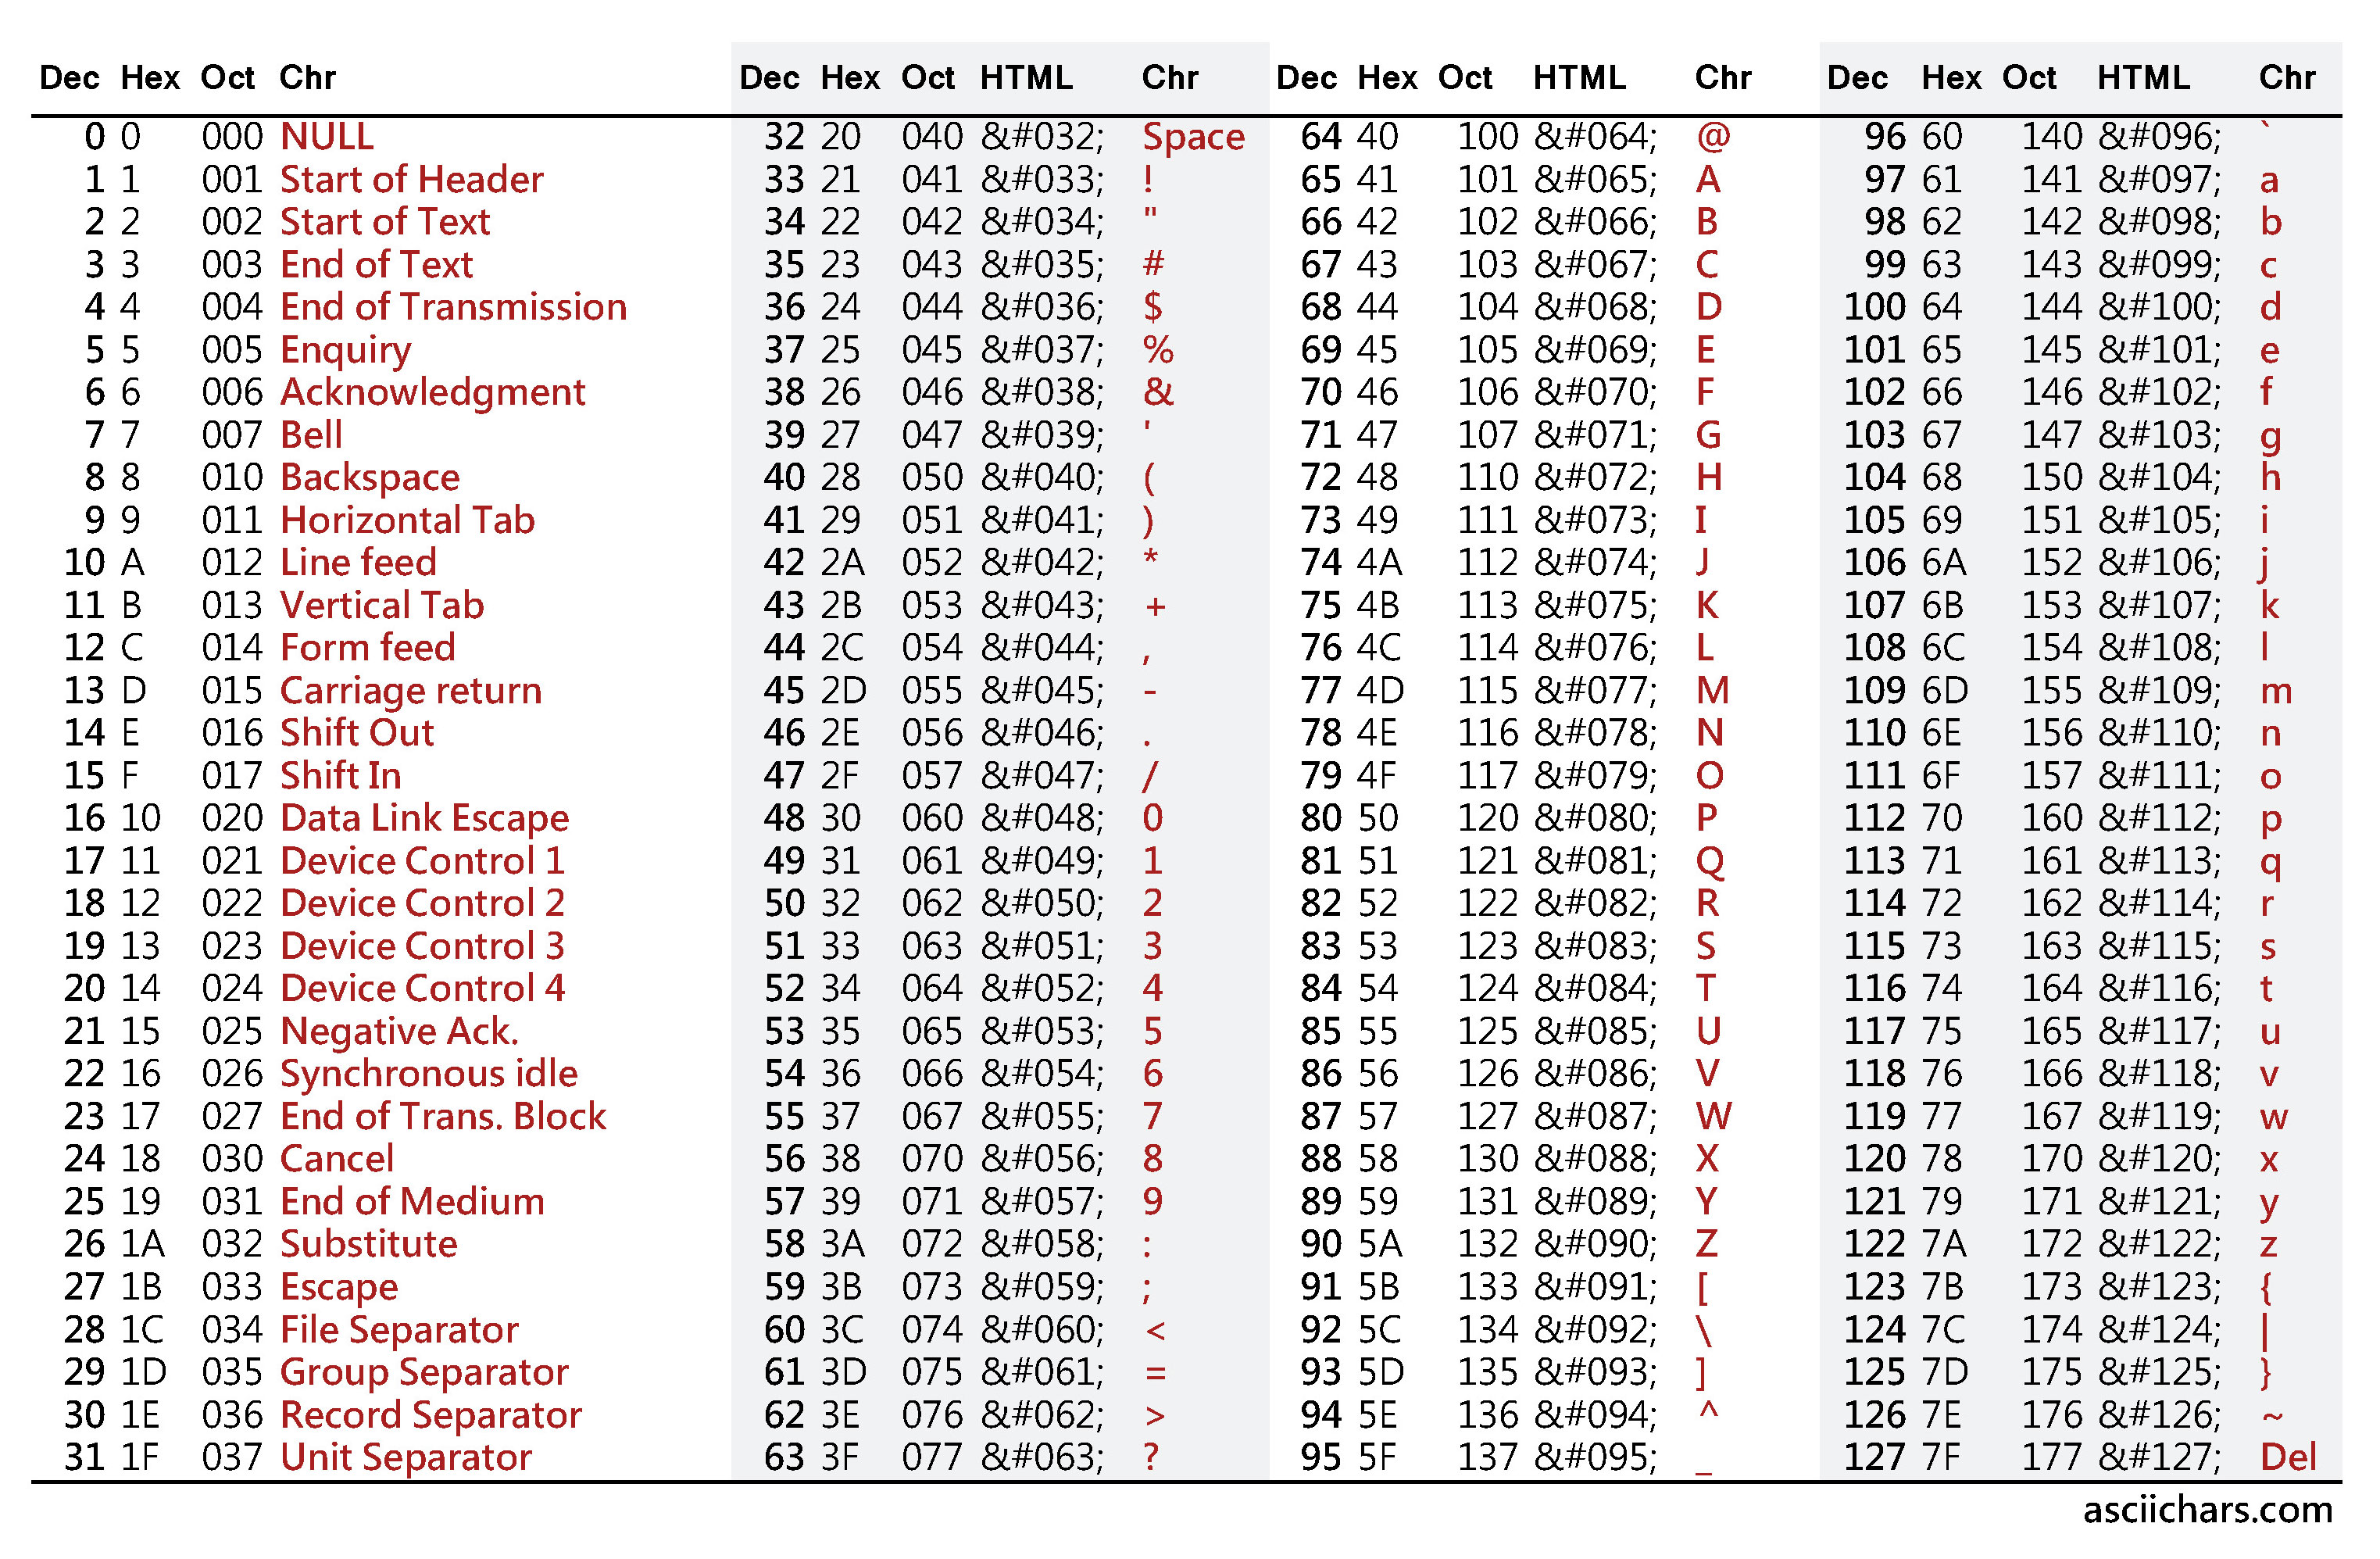
\includegraphics[width=1\textwidth]{figures/ASCII.JPG}}
\caption{tampilan tabel ASCII}
\label{ASCII}
\end{figure}

%UTF-8
	\section{UTF-8}
	 berdasarkan artikel yang ditulis oleh yergeau menyatakan bahwa \cite{yergeau1996utf}
		UTF-8 didefinisikan oleh Unicode Standard [UNICODE]. Deskripsi dan
   Rumus juga dapat ditemukan pada Lampiran D dari ISO / IEC 10646-1 [ISO.10646]

   Dalam UTF-8, karakter dari rentang U + 0000..U + 10FFFF (UTF-16
   jangkauan yang mudah diakses) dikodekan menggunakan urutan 1 sampai 4 oktet. Itu
   hanya oktet dari "urutan" satu memiliki bit orde tinggi yang diset ke 0,
   7 bit sisanya digunakan untuk mengkodekan nomor karakter. Di sebuah
   urutan n oktet, n> 1, oktet awal memiliki n orde tinggi
   bit set ke 1, diikuti oleh bit set ke 0. Bit yang tersisa dari
   oktet itu berisi bit dari jumlah karakter yang akan ada
   dikodekan Berikut oktet (s) semua memiliki bit orde tinggi yang disetel
   1 dan bit berikut diset ke 0, meninggalkan 6 bit di masing-masing berisi
   bit dari karakter yang akan dikodekan.

   Tabel di bawah merangkum format jenis oktet yang berbeda ini.
   Huruf x menunjukkan bit yang tersedia untuk mengkodekan bit dari
   nomor karakter.
 \begin{table}[H]
 \begin{tabular}{|c|c|c}
 hline
 Arang. rentang angka & Urutan oktet UTF-8
 (heksadesimal) & (biner)\\
 \hline
 0000 0000-0000 007F & 0xxxxxxx\\
 0000 0080-0000 07FF & 110xxxxx 10xxxxxx\\
 0000 0800-0000 FFFF & 1110xxxx 10xxxxxx 10xxxxxx\\
 0001 0000-0010 FFFF & 11110xxx 10xxxxxx 10xxxxxx 10xxxxxx\\
\hline
\end{tabular}
\end{table}

   Pengkodean karakter ke UTF-8 berlangsung sebagai berikut:
   \begin{enumerate}
   	\item Tentukan jumlah oktet yang dibutuhkan dari nomor karakter
       dan kolom pertama dari tabel di atas. Penting untuk dicatat
       bahwa baris tabel saling eksklusif, yaitu, ada
       hanya satu cara yang valid untuk mengkodekan karakter tertentu.
    \item Siapkan bit orde tinggi dari oktet per detik
       kolom meja
    \item Isi bit yang ditandai x dari bit dari nomor karakter,
       dinyatakan dalam biner Mulailah dengan meletakkan bit dengan urutan terendah
       nomor karakter pada posisi paling rendah dari yang terakhir
       octet dari urutan, kemudian menempatkan bit urutan yang lebih tinggi berikutnya
       nomor karakter di posisi orde tinggi berikutnya dari oktet tersebut,
       dll. Bila bit x dari oktet terakhir terisi, lanjutkan ke
       berikutnya sampai oktet terakhir, lalu ke yang sebelumnya, dll sampai semuanya
       x bit terisi.
    \end{enumerate}

    Definisi UTF-8 melarang pengkodean nomor karakter antara
   U + D800 dan U + DFFF, yang dicadangkan untuk penggunaan dengan UTF-16
   bentuk pengkodean (sebagai pasangan pengganti) dan tidak secara langsung mewakili
   karakter. Saat mengkodekan dalam UTF-8 dari data UTF-16, diperlukan
   untuk pertama memecahkan kode data UTF-16 untuk mendapatkan nomor karakter, yang
   kemudian dikodekan dalam UTF-8 seperti dijelaskan di atas. Ini kontras dengan
   CESU-8 [CESU-8], yang merupakan pengkodean UTF-8-like yang tidak dimaksudkan untuk
   gunakan di Internet CESU-8 beroperasi serupa dengan UTF-8 namun mengkodekan
   nilai kode UTF-16 (jumlah 16 bit) bukan karakternya
   nomor (kode titik). Hal ini menyebabkan hasil yang berbeda untuk karakter
   angka di atas 0xFFFF; pengkodean CESU-8 dari karakter tersebut TIDAK
   UTF-8 yang valid

   Decoding karakter UTF-8 akan menghasilkan sebagai berikut:
   \begin{enumerate}
   \item Inisialisasi bilangan biner dengan semua bit diset ke 0. Hingga 21 bit
       mungkin dibutuhkan

   \item Tentukan bit yang mengkodekan nomor karakter dari nomor tersebut
       dari oktet di urutan dan kolom kedua dari tabel
       di atas (bit ditandai x).

   \item Bagikan bit dari urutan ke bilangan biner, pertama
       bit orde rendah dari oktet terakhir dari urutan dan
       melanjutkan ke kiri sampai tidak ada x bit yang tertinggal. Biner
       nomor sekarang sama dengan nomor karakter.
    \end{enumerate}
   Implementasi algoritma decoding di atas HARUS melindungi terhadap
   decoding invalid sequence. Misalnya, sebuah implementasi naif mungkin
   decode urutan UTF-8 yang terlalu lama C0 80 ke karakter U + 0000,
   atau pasangan pengganti ED A1 8C ED BE B4 ke U + 233B4. Decoding
   urutan yang tidak valid mungkin memiliki konsekuensi keamanan atau penyebab lainnya
   masalah. Lihat Pertimbangan Keamanan (Bagian 10) di bawah ini.

	\subsection{Byte order mark (BOM)}
   Karakter UCS U + FEFF "ZERO WIDTH NO-BREAK SPACE" juga dikenal
   secara informal sebagai "BYTE ORDER MARK" (disingkat "BOM"). Karakter ini
   dapat digunakan sebagai "RUANG BAWAH TANPA BREAK" NOL yang asli "dalam teks, tapi
   nama BOM mengisyaratkan kemungkinan penggunaan karakter yang kedua: untuk
   menambahkan karakter U + FEFF ke aliran karakter UCS sebagai a
   "tanda tangan". Penerima aliran serial seperti itu kemudian dapat menggunakan
   karakter awal sebagai petunjuk bahwa aliran terdiri dari UCS
   karakter dan juga untuk mengenali pengkodean UCS mana yang terlibat dan,
   dengan pengkodean yang memiliki unit pengkodean multi-oktet, sebagai cara untuk mengenali urutan serialisasi dari oktet tersebut. UTF-8 memiliki a
   unit pengkodean single-oktet, fungsi terakhir ini tidak ada gunanya dan BOM
   akan selalu tampil sebagai urutan oktet BB BB BF.

Sementara itu, ketidakpastian sayangnya tetap dan mungkin akan mempengaruhi
   Protokol internet Spesifikasi protokol MUNGKIN membatasi penggunaan
   U + FEFF sebagai tanda tangan untuk mengurangi atau menghilangkan potensi
   efek buruk dari ketidakpastian ini. Demi kepentingan mogok a
   keseimbangan antara keuntungan (pengurangan ketidakpastian) dan
   Kekurangan (kehilangan fungsi tanda tangan) dari pembatasan tersebut, itu
   berguna untuk membedakan beberapa kasus:

    1. Protokol HARUS melarang penggunaan U + FEFF sebagai tanda tangan untuk itu
      elemen protokol tekstual yang mandat protokolnya selalu
      UTF-8, fungsi tanda tangan sama sekali tidak berguna bagi mereka
      kasus.

    2. Protokol HARUS melarang penggunaan U + FEFF sebagai tanda tangan untuk
      elemen protokol teks yang disediakan oleh protokol ini
      mekanisme identifikasi pengkodean karakter, bila diharapkan
      bahwa implementasi protokol akan berada dalam posisi untuk
      selalu gunakan mekanisme dengan benar. Ini akan terjadi kapan
	  3. elemen protokol dipelihara dengan ketat di bawah kendali
      pelaksanaannya mulai dari saat penciptaan sampai saat ini
      transmisi mereka (diberi label dengan benar).

    4. Protokol TIDAK HARUS melarang penggunaan U + FEFF sebagai tanda tangan
      elemen protokol tekstual yang protokolnya tidak
      berikan mekanisme identifikasi pengkodean karakter, bila ada larangan
      tidak dapat dijalankan, atau bila diharapkan begitu
      Implementasi protokol tidak akan berada dalam posisi
      selalu gunakan mekanisme dengan benar. Dua kasus terakhir adalah
      Kemungkinan besar terjadi dengan elemen protokol yang lebih besar seperti MIME
      entitas, terutama bila implementasi protokol akan dilakukan
      Dapatkan entitas semacam itu dari sistem file, dari protokol yang tidak
      memiliki mekanisme identifikasi encoding untuk muatan (seperti FTP)
      atau dari protokol lain yang tidak menjamin tepat
      identifikasi pengkodean karakter (seperti HTTP).
     hal tersebut berdasarkan yang ditulis dalam artikel wahl \cite{wahl1997lightweight}